%!TEX program = xelatex
%!TEX TS-program = xelatex
%!TEX encoding = UTF-8 Unicode

\documentclass[12pt, a4paper]{article}
\usepackage{CJKutf8}
\usepackage{graphicx}
\usepackage{subfigure}
\usepackage{listings}
\usepackage[colorlinks,linkcolor=blue]{hyperref}
\usepackage{ulem}
\usepackage{xcolor}
\usepackage{caption2}
\usepackage{amssymb}
\usepackage{indentfirst} % 中文段落首行缩进
\setlength{\parskip}{0.5em}
\renewcommand{\figurename}{图} % 将图表的标题设置为中文“图”

\title{第十八·逆向选择·信息不对称与道德风险}
\author{hoochanlon}
\date{\today}

\begin{document}
	\begin{CJK*}{UTF8}{gbsn}
		\maketitle
        \clearpage
        \section{信息差异}

        \subsection{完全信息和不完全信息}
        参与者的集合、行动顺序、策略空间、信息空间,以及损益函数,这些如果都是参与人的共同知识。那么这个博弈就是完全信息博弈。
        反之,如果参与者的信息空间不同,那么这个博弈就是不完全信息博弈。

        \subsection{完全信息博弈均衡求解}
        爱惜钱财的父母面对残暴型绑匪的一个策略表达式:
        \begin{itemize}
            \item 对于父母来说,不付赎金为占优策略。对于绑匪来说,撕票为占优策略。
            \item 父母不付赎金,绑匪撕票。就是这个博弈的占优策略纳什均衡,但这个结果并非双方最优。
            \item 父母:父母不付赎金,绑匪放人,最优;绑匪:付完赎金撕票,最优。
        \end{itemize}

        \begin{figure}[htbp]
            \centering
            \subfigure[残暴型绑匪博弈]{
                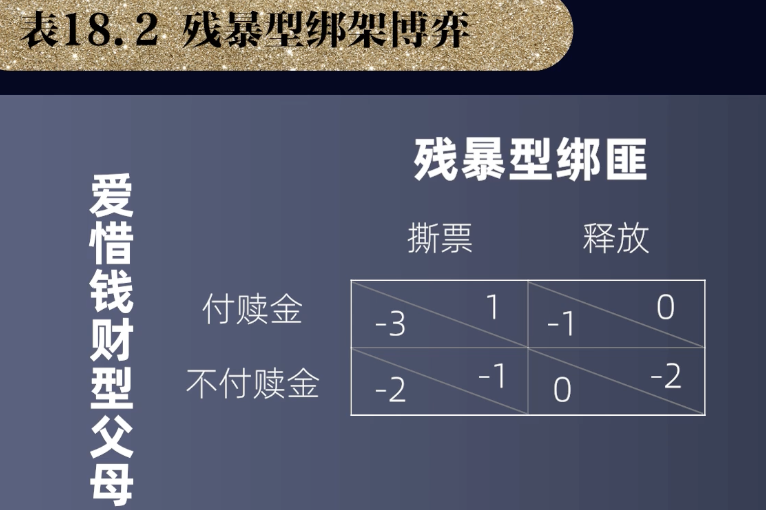
\includegraphics[width=0.46\textwidth]{./figures/catch2023-08-02-14.49.50.png}
            }
            \subfigure[金钱至上型绑匪博弈]{
                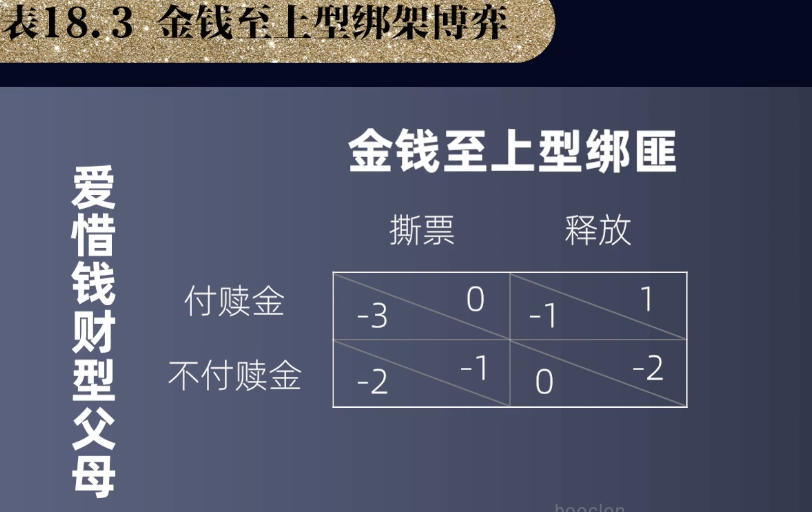
\includegraphics[width=0.46\textwidth]{./figures/catch2023-08-02-14.57.52.png}
            }
        \end{figure}

        \subsection{绑架博弈(动态博弈)}
        \textbf{静态博弈中,我们是根据对对方策略,选择的想象,预判和推测,然后做出我的最优策略选择。
        \textcolor{red}{而动态博弈是后行动的参与者会根据先行动者的实际行动结果,我再做出对于我来说最优的选择。}} \par
        因此对于绑匪来说他是存在四种策略选择:
        \begin{itemize}
            \item 无论父母是否支付赎金一律撕票
            \item 无论父母是否支付赎金一律释放人质
            \item 如果收到钱,就释放人质;如果没有收到钱,就撕票。
            \item 如果收到钱,就撕票;如果没有收到钱,就释放人质。
        \end{itemize}
        策略其实是从信息到行动的全部映射关系,所以它会包含所有可能情况下面的所有的行动计划。在动态的绑架博弈中,那么双方博弈的完整的策略表达式:

        \begin{figure}[htbp]
            \centering
            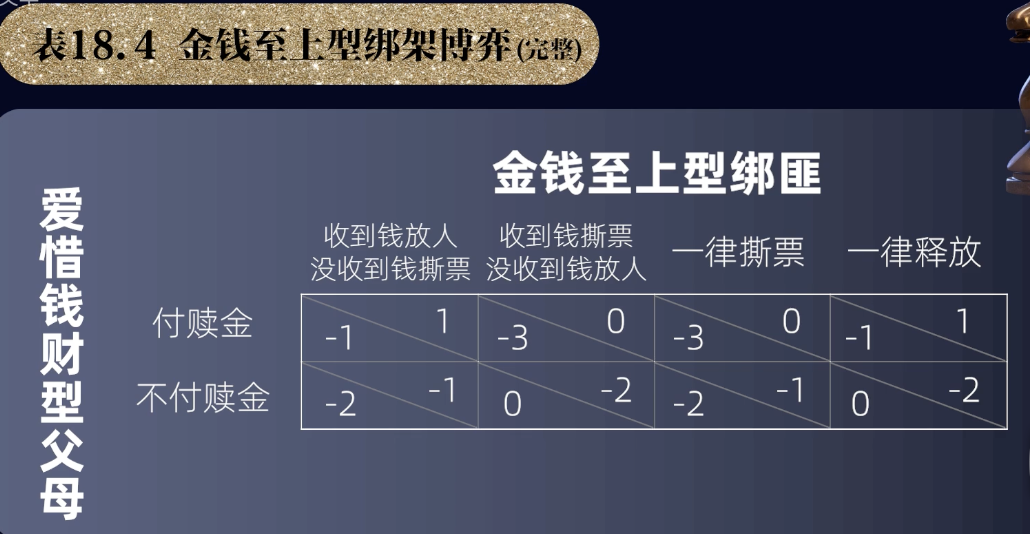
\includegraphics[width=0.8\textwidth]{./figures/catch2023-08-02-15.29.21.png}
        \end{figure}

        在动态博弈中父母是没有占优策略的,如果父母预期绑匪的策略是“收到钱,我放人;没收钱,我撕票”,那么父母就会发现我选择付赎金对我最有利。
        如果父母预期到绑匪是另外三种策略,父母自然会选择不付赎金了。对于金钱至上的绑匪不管有没有付赎金都选择撕票,虽然是纳什均衡,但其实是劣策略,
        并非子博弈的完美纳什均衡。\par
        满足子博弈完美纳什均衡满足条件:
        \begin{enumerate}
            \item 该策略组合是整个博弈的纳什均衡。
            \item 该策略组合在每个子博弈是纳什均衡。
        \end{enumerate}
        没收到钱,撕票;收到钱后,放人。这个策略组合是整个博弈的纳什均衡,也是每个子博弈的纳什均衡。因此这个策略组合就是子博弈完美纳什均衡。
        \subsubsection{不完全信息博弈均衡求解}
        不完全信息博弈的四种结果
        \begin{enumerate}
            \item 父母以为绑匪是金钱至上型,选择支付赎金,实际绑匪是残暴型,导致人财两空,损益为了-3。
            \item 父母以为绑匪是金钱至上型,选择支付赎金,实际判断正确,绑匪释放了人质,损益为-1。
            \item 父母以为绑匪是残暴型,选择不付赎金,实际绑匪确实是残暴型,损益为-2。
            \item 父母以为绑匪是残暴的,选择不付赎金,实际绑匪是金钱至上型,损益为-2。
        \end{enumerate}
        父母支付赎金不取决于绑匪的类型,而取决于父母对绑匪类型的猜测。比如马路边有人问你讨5块钱,取决于你认为他是不是骗子。因此对于参与人类型的判断,
        取决于信念(belief),那么在不完全信息的博弈中,你对他人的信念决定了你当下的选择。

        \subsection{绑架中的逆向选择}
        当父母相信绑匪残暴的概率大于50\%的时候,其实绑匪的最佳策略是不绑架;当金钱至上的概率大于50\%,绑匪的最佳策略是绑架。无论他确实是残暴的,
        还是金钱至上的。那么父母对绑匪的信念,决定了绑匪的行为选择。\textbf{ 换句话说,绑匪只绑架那些更愿意相信他是金钱至上的父母的孩子,
        就像骗子只骗那些不相信他是骗子的人,这就会带来逆向选择。\textcolor{red}{你越相信对方是善良的,对方越容易骗你。因此你越来越不敢相信对方是善良的,
       相信绑匪是残暴型的父母的比例就会上升,这样的结果,不仅仅这个残暴的绑匪赚不到钱,金钱至上的绑匪也驱逐出市场了。}}\par

       \clearpage
       \section{阿克洛夫的贡献}
       \subsection{劣币驱逐良币}
       逆向选择最早叫格雷欣法则或叫劣币驱逐良币,两种实际价值不同而名义价值相同的货币同时流通时,实际价值较高的货币,即所谓的良币,会被收藏、熔化或被输出国外,从而退出流通。
       在市场上广泛流通的都是那些实际价值较低的货币,即所谓的劣币。 \par
       阿克洛夫《柠檬市场:质量的不确定性与市场机制》指出二手车市场作为质量不确定性的一个例子,用经济学的方法分析,就是二手车市场交易中的逆向选择问题。
       柠檬市场指的是一种买卖双方信息不对称,导致的低质量的商品大行其道的市场。车主往往比买家拥有更多的车辆信息,当买家无法确定某俩二手车的真实的品质质量的时候,那么只能以其对所有该类型二手车的平均的质量来付费。
       \begin{quote}
        {\small 买到低品质的就亏了,高品质的也就赚了;问题是卖家知道自己的车是高品质还是低品质,那么高品质的没得赚,自然也不会去卖了。那当然买家也不傻,只要愿意卖的,品质也不会高于6万以上,肯定是低品质的了。那这样的话,买家也不愿意出6万,6万买到的高品质几乎没有,那只有低品质的可能性。最后他也只愿意出4万买。}
        \end{quote}
        当商品卖方对商品的质量状况,拥有比买方更多信息的时候,市场交易将受这种不对称信息的影响,导致质量较高的商品,不断退出这个市场,而质量较差的商品,逐步占领这个市场。这就出现了逆向选择的现象。

        \clearpage
        \section{无处不在的逆淘汰}
        其实一般而言,在产品市场里面,往往是高质量高价,低质量低价,满足不同消费者对不同品质的需求。那么随着人们收入水平不断提升,人们对高品质产品的需求会增加,对低品质的产品的需求会减少。因此总体而言,高品质产品在市场上面的比例,总体是不断上升的。\textbf{然而在信息不对称的情况下面,我们也能够看到大量的逆淘汰现象。}
        \subsection{信贷市场和一般产品市场的不同}
        信贷配给:借100万,但银行往往只给50万,借钱人往往比银行更清楚自己的还款能力,这里就有信息不对称。收益不仅取决于利息,还取决于你的还款能力。
        当贷款利率上升时,低风险的借款人会被高风险借款人所淘汰。因此为了避免出现逆淘汰,银行就给出低于市场均衡的利率,然后再评估借款人的还款能力的基础上面,有选择性的放贷。
        \begin{enumerate}
            \item 信贷市场不遵守“价高者得”的交易原则。
            \item 信贷市场不遵守“多多益善”的销售原则。
        \end{enumerate}
        由于信息不对称的广泛存在,也导致生活中出现各种各样的逆淘汰。西安做为是十三朝古都,有着悠久的历史沉淀,可这样的市场古玩真品率是5~8\%,这还是全国最高的,其他地方的市场可想而知。在单方面的想象中,一开始的古玩市场出售的基本上可能是真品为主,卖家以假乱真能够暴赚一笔,而买家也不傻,当知道他以假乱真的时候,那么他就只愿意出一个更低的价格,这样以来卖家即使有真品,也自己收藏着了。

    \end{CJK*}
\end{document}
